\begin{figure}
    \centering
    \begin{minipage}{0.45\textwidth}
        \centering
        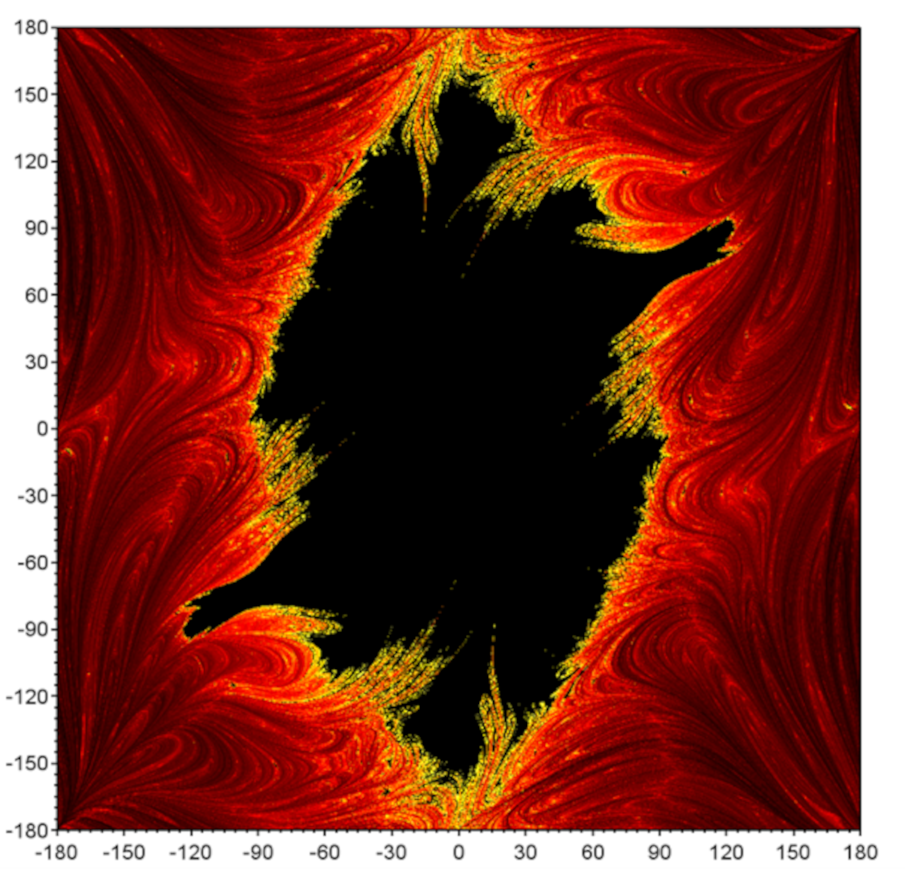
\includegraphics[width=\textwidth]{papers/doppelpendel/images/parameterraum.png}
    \end{minipage}
    \hfill
    \begin{minipage}{0.45\textwidth}
        \centering
        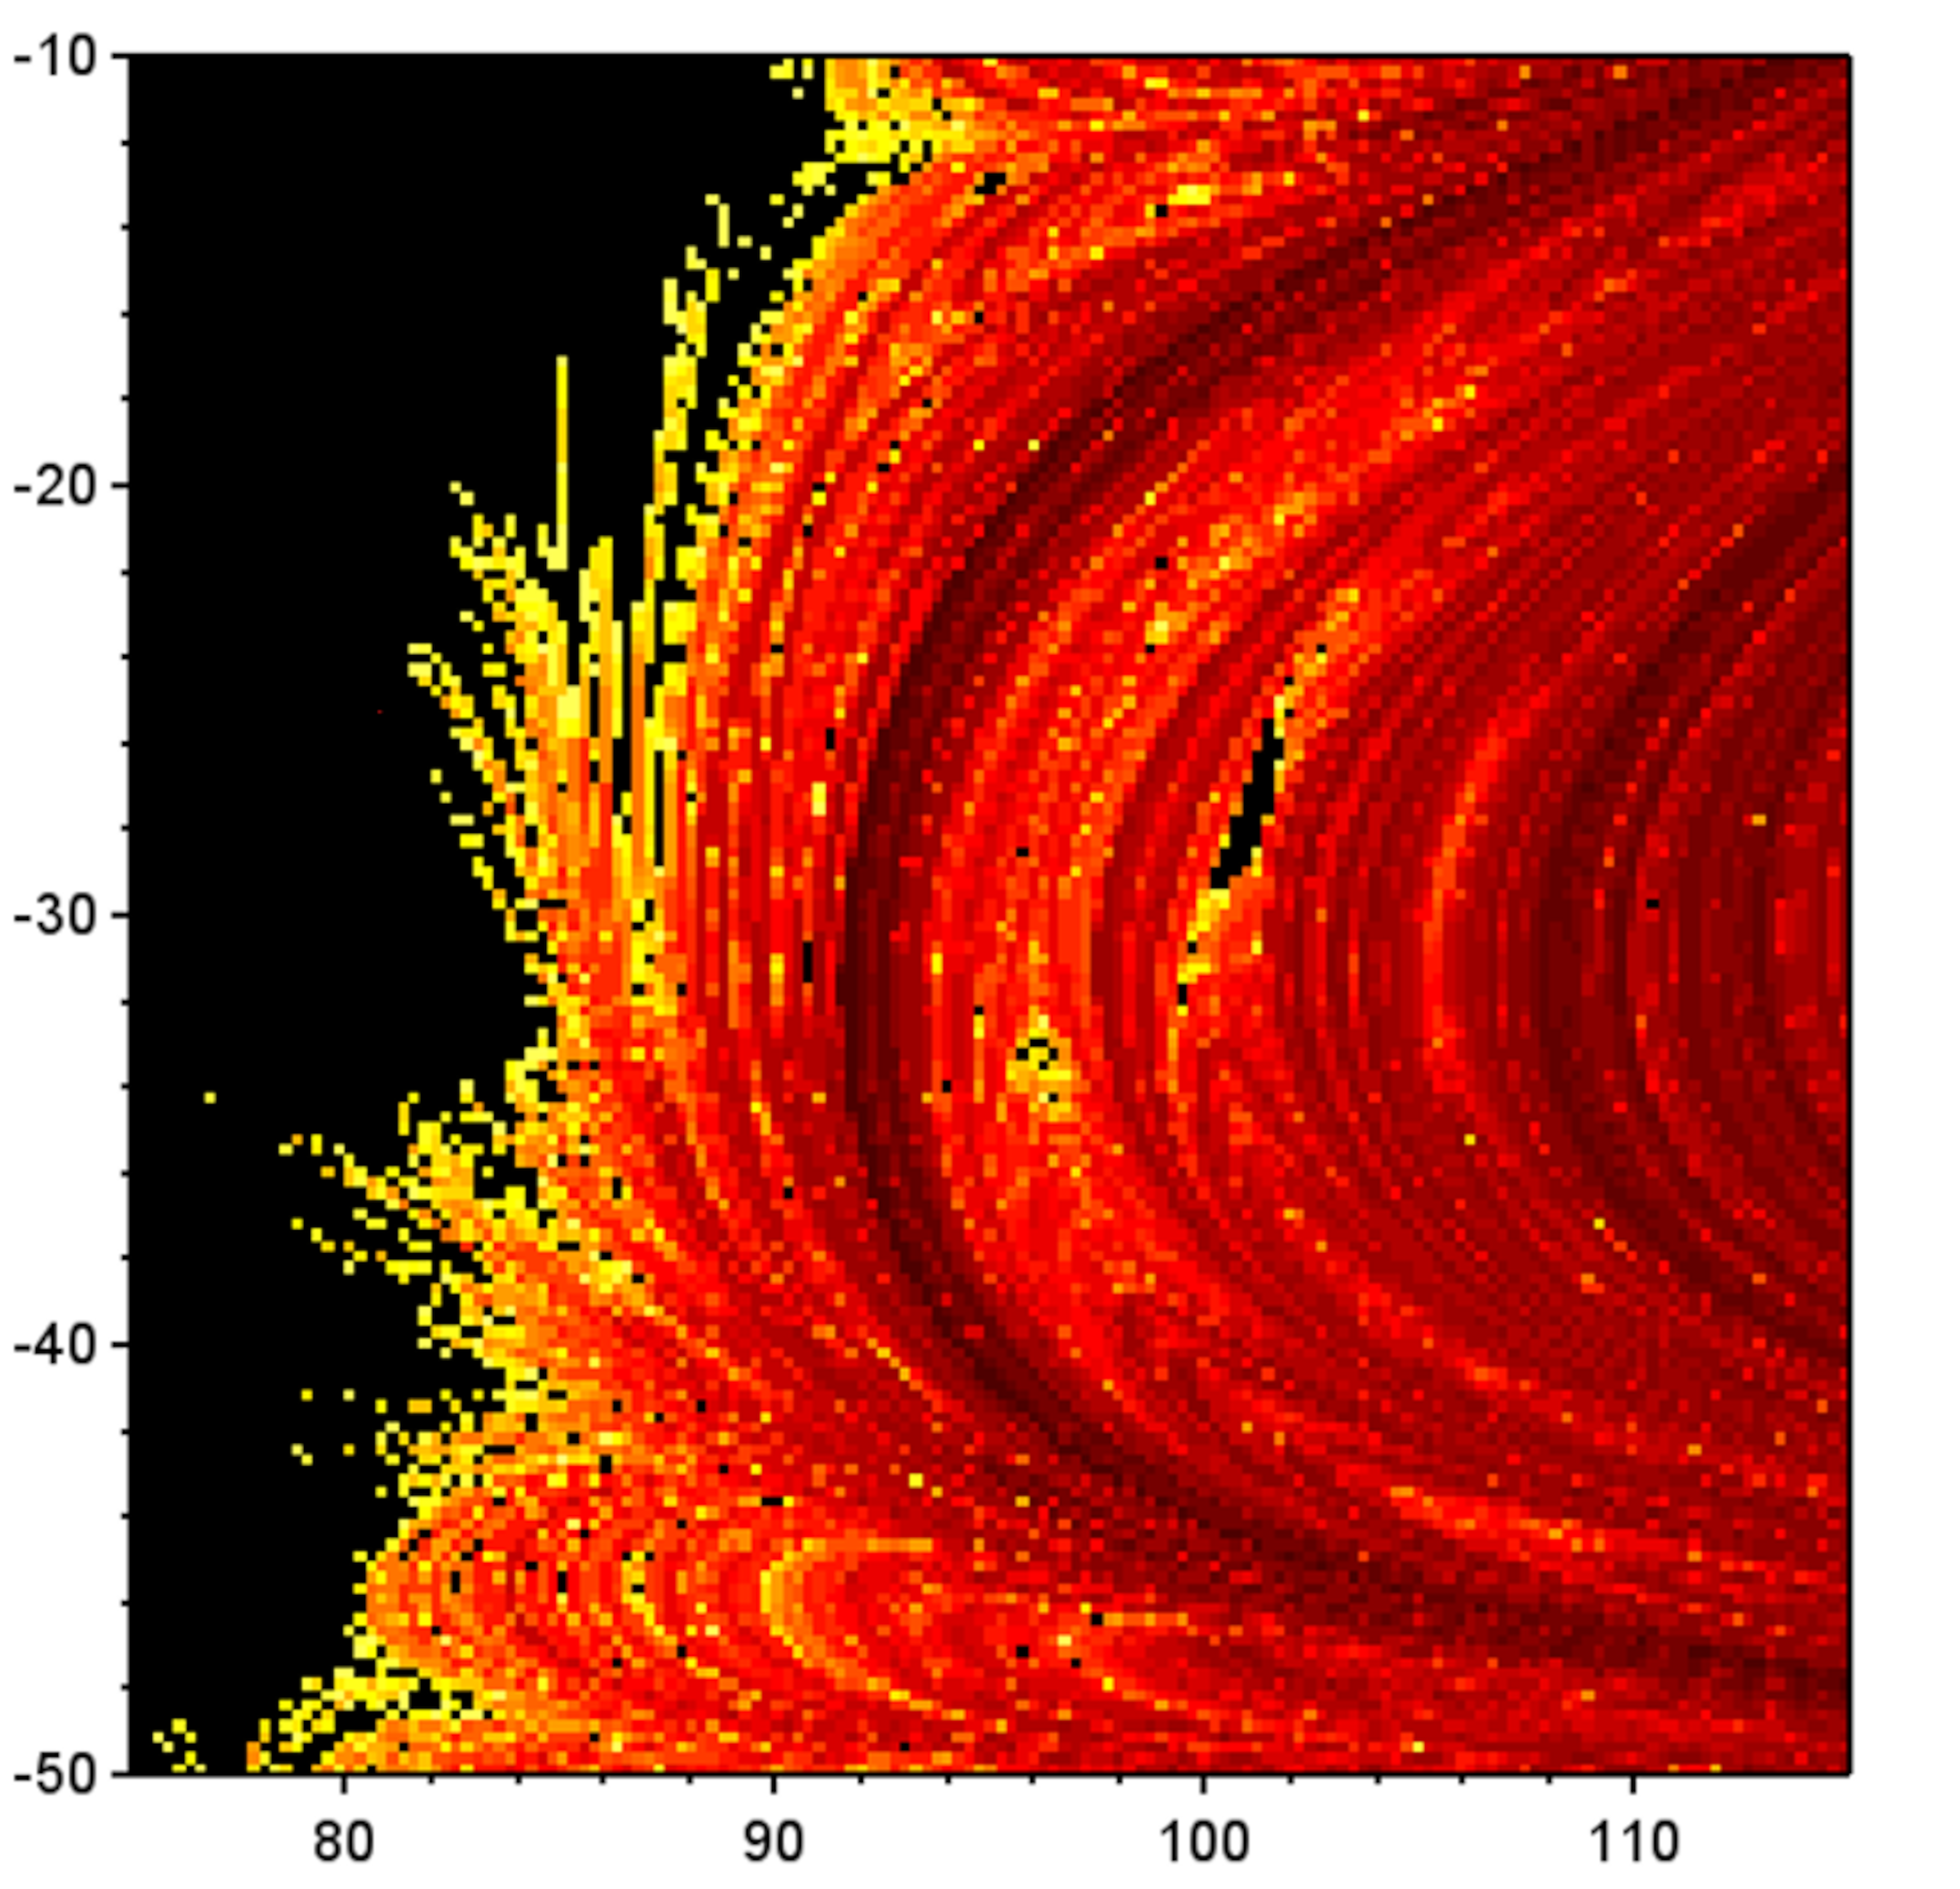
\includegraphics[width=\textwidth]{papers/doppelpendel/images/parameterraum_stabile_inseln.png}
    \end{minipage}
    \caption{Winkelpaare im Parameterraum (links) und stabile Inseln im Parameterraum (rechts)
    \cite{doppelpendel:wettbewerbsarbeit}}
    \label{fig:Parameterraum}
\end{figure}
